% Gemini theme
% https://github.com/anishathalye/gemini

\documentclass[final]{beamer}

% ====================
% Packages
% ====================

\usepackage[T1]{fontenc}
\usepackage{lmodern}
\usepackage[size=custom,width=120,height=72,scale=1.0]{beamerposter}
\usetheme{gemini}
\usecolortheme{gemini}
\usepackage{graphicx}
\usepackage{booktabs}
\usepackage{setspace}

% Bibliography setting
\usepackage{paralist}
\usepackage{xpatch}
\usepackage[style=numeric]{biblatex}
\addbibresource{poster.bib}

\usepackage{tikz, pgfplots}

\usetikzlibrary{
    arrows.meta,
    calc,
    decorations,
    decorations.pathreplacing,
    decorations.footprints,
    math,
    patterns,
    shadows,
    external
}

\tikzexternalize

\tikzset{>=stealth}

\pgfplotsset{compat=1.16}

\usepgfplotslibrary{
    polar,
    colormaps,
    colorbrewer,
    groupplots,
    statistics
}

\newcommand{\inputtikz}[1]{%
  \tikzsetnextfilename{#1}%
  \input{#1.tikz}%
}

\newcommand{\doublec}[2]{% double diffusion arrows
  \draw  [-Circle] ($(#1.north east)!0.7!(#1.north)$) -- ($(#2.south east)!0.7!(#2.south)$);
  \draw  [Circle-] ($(#1.north west)!0.7!(#1.north)$) -- ($(#2.south west)!0.7!(#2.south)$);
  }


\newcommand{\singlec}[2]{% single diffusion arrows
  \draw [-Latex] (#1.east) -- (#2.west);
  }

% Set the TikZ neuron style up, since it's used many times
\tikzset{
  neuron/.style={
  % The shape:
  circle,
  % The size:
  minimum size=6mm,
  % The border:
  very thick,
  draw=blue!50!black!50,
  % The filling:
  top color=white,
  bottom color=blue!50!black!20, % and something else at the bottom
  % Font
  font=\itshape,
  % padding around node
  outer sep=2mm
  }
}

\usepackage[siunitx]{circuitikzgit}

\ctikzset{bipoles/length=1cm}

% ====================
% Lengths
% ====================

% If you have N columns, choose \sepwidth and \colwidth such that
% (N+1)*\sepwidth + N*\colwidth = \paperwidth
\newlength{\sepwidth}
\newlength{\colwidth}
\setlength{\sepwidth}{0.025\paperwidth}
\setlength{\colwidth}{0.3\paperwidth}

\newcommand{\separatorcolumn}{\begin{column}{\sepwidth}\end{column}}

% ====================
% Title
% ====================

\title{A minimal reaction-diffusion neural model generates {\emph{C. elegans}} undulation}

\author{Anshul Singhvi \inst{1, 3} \and Harold Hastings \inst{1} \and Jenny Magnes \inst{2} \and Cheris Congo \inst{2} \and Miranda Hulsey-Vincent \inst{2} \and Rifah Tasnim \inst{1} \and Naol Negassa \inst{1}}

\institute[shortinst]{\inst{1} Bard College at Simon's Rock \samelineand \inst{2} Vassar University \samelineand \inst{3} Columbia University}

% ====================
% Footer (optional)
% ====================

\footercontent{
  \href{https://youtu.be/5327kroOwCk}{See the APS March Meeting talk on YouTube} \hfill
  International Physics of Living Systems, 2020 \hfill
  \href{mailto:asinghvi17@simons-rock.edu}{asinghvi17@simons-rock.edu}}
% (can be left out to remove footer)

% ====================
% Logo (optional)
% ====================

% use this to include logos on the left and/or right side of the header:
\logoleft{ 
\includegraphics[width=13cm]{figures/logos/sr.pdf}}
\logoright{
\includegraphics[width=13cm]{figures/logos/vassar.pdf}}


% ====================
% Body
% ====================

\begin{document}

\linespread{1.2}

\begin{frame}[t]
\begin{columns}[t]
\separatorcolumn

\begin{column}{\colwidth}

  \begin{block}{Abstract}

      The small (1 mm) nematode \emph{Caenorhabditis elegans} has become widely used as a model organism; in particular the \emph{C. elegans} connectome has been completely mapped, and \emph{C. elegans} locomotion has been widely studied (c.f. http://www.wormbook.org). We describe a minimal reaction-diffusion model for the \emph{C. elegans}. This may be considered a simple model for Xu et al.'s "descending pathway" description of the \emph{C. elegans} central pattern generator (CPG) \cite{xu2018}. Olivares \emph{et al} \cite{olivares2019} present a likely more realistic model which relies on small networks of neurons, and presents a distributed model of the CPG. In particular, we use simulation methods to show that a small network of FitzHugh-Nagumo neurons (one of the simplest neuronal models) can generate key features of \emph{C. elegans} undulation, and thus locomotion.  Finally, we recreate the required oscillations and coupling with a network of coupled Keener \cite{keener1983} analog neurons.

  \end{block}

  \begin{block}{The FitzHugh-Nagumo model}
      The FitzHugh-Nagumo equations have the form:
      \[
      \begin{aligned}
        &\frac{d v}{d t} = f(v) - w + I_{ext} + \color{forestgreen}{D \cdot (v_\mathrm{driving} - v)}\\
        &\frac{d w}{d t} = \epsilon(v - \gamma w + \beta)\\
        &f(v) = v - \frac{v^3}{3}
      \end{aligned}
      \]
      where $v$ is the membrane potential, $w$ is a slow inhibitor variable, AND $\epsilon$, $\gamma$ and $\beta$ are constants.  It turns out that $f(v)$ can be any cubic-like function which sufficiently approximates $v - \frac{v^3}{3}$.

      A method for diffusive inter-neuron coupling has been introduced in green.  $D$ is the diffusion coefficient, and can be positive (excitatory synapses, gap junctions) or negative (inhibitory junctions).  The quantity scaled by $D$ is simply the voltage difference between the driving neuron and the driven one.

  \end{block}

  \begin{block}{The central pattern generator}

        \textit{Caenorhabditis elegans} is a small nematode with a well-known neuronal layout.  Its central pattern generator can be sufficiently approximated by a simple neuronal network, arranged as such:

        \begin{figure}
            \centering
            \inputtikz{figures/cpg/cpg}
            \caption{The central pattern generator, simplified.}
        \end{figure}
        % \begin{minipage}[b]{0.15\pagewidth}
        %     \begin{figure}
        %         \centering
        %         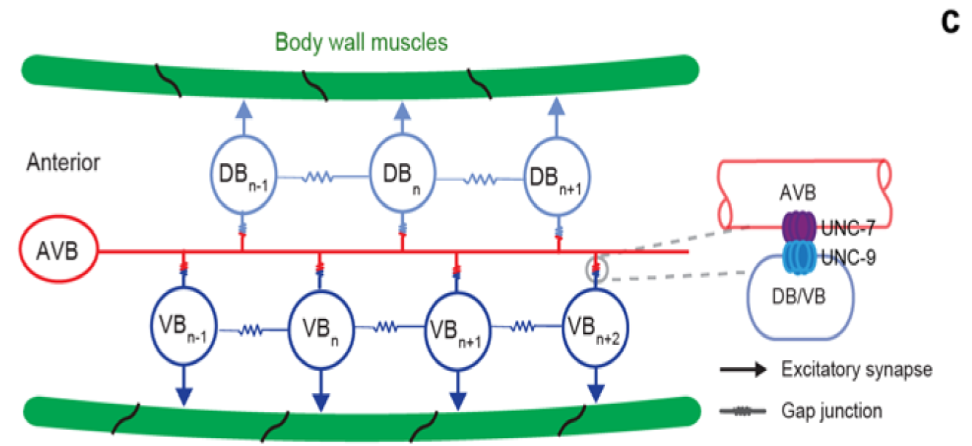
\includegraphics{figures/xu_cpg.png}
        %         \caption{CPG from Xu \textit{et al} \cite{xu2018}.}
        %     \end{figure}
        % \end{minipage}

        wherein \tikz[scale=.68, every node/.style={scale=.6}]{\node (0) [neuron] at (0, 0) {0};\node (1) [neuron] at (3, 0) {1};\draw [-Latex] (0.east) -- (1.west);} represents unidirectional diffusion coupling, and \tikz[scale=.68, every node/.style={scale=.6}]{\node (0) [neuron] at (0, 0) {0}; \node (1) [neuron] at (3, 0) {1}; \draw [-Circle] ($(0.north east)!0.7!(0.east)$) -- ($(1.north west)!0.7!(1.west)$); \draw [Circle-] ($(0.south east)!0.7!(0.east)$) -- ($(1.south west)!0.7!(1.west)$);} represents bidirectional diffusion coupling.

  \end{block}

\end{column}

\separatorcolumn

\begin{column}{\colwidth}

  \begin{block}{Simulation and experimental data}

    Vivamus congue volutpat elit non semper. Praesent molestie nec erat ac
    interdum. In quis suscipit erat. \textbf{Phasellus mauris felis, molestie
    ac pharetra quis}, tempus nec ante. Donec finibus ante vel purus mollis
    fermentum. Sed felis mi, pharetra eget nibh a, feugiat eleifend dolor. Nam
    mollis condimentum purus quis sodales. Nullam eu felis eu nulla eleifend
    bibendum nec eu lorem. Vivamus felis velit, volutpat ut facilisis ac,
    commodo in metus.

    \begin{enumerate}
      \item \textbf{Morbi mauris purus}, egestas at vehicula et, convallis
        accumsan orci. Orci varius natoque penatibus et magnis dis parturient
        montes, nascetur ridiculus mus.
      \item \textbf{Cras vehicula blandit urna ut maximus}. Aliquam blandit nec
        massa ac sollicitudin. Curabitur cursus, metus nec imperdiet bibendum,
        velit lectus faucibus dolor, quis gravida metus mauris gravida turpis.
      \item \textbf{Vestibulum et massa diam}. Phasellus fermentum augue non
        nulla accumsan, non rhoncus lectus condimentum.
    \end{enumerate}

  \end{block}

  \begin{block}{Fusce aliquam magna velit}

    Et rutrum ex euismod vel. Pellentesque ultricies, velit in fermentum
    vestibulum, lectus nisi pretium nibh, sit amet aliquam lectus augue vel
    velit. Suspendisse rhoncus massa porttitor augue feugiat molestie. Sed
    molestie ut orci nec malesuada. Sed ultricies feugiat est fringilla
    posuere.

    \begin{figure}
      \centering
      \begin{tikzpicture}
        \begin{axis}[
            scale only axis,
            no markers,
            domain=0:2*pi,
            samples=100,
            axis lines=center,
            axis line style={-},
            ticks=none]
          \addplot[red] {sin(deg(x))};
          \addplot[blue] {cos(deg(x))};
        \end{axis}
      \end{tikzpicture}
      \caption{Another figure caption.}
    \end{figure}

  \end{block}

  \begin{block}{Nam cursus consequat egestas}

    Nulla eget sem quam. Ut aliquam volutpat nisi vestibulum convallis. Nunc a
    lectus et eros facilisis hendrerit eu non urna. Interdum et malesuada fames
    ac ante \textit{ipsum primis} in faucibus. Etiam sit amet velit eget sem
    euismod tristique. Praesent enim erat, porta vel mattis sed, pharetra sed
    ipsum. Morbi commodo condimentum massa, \textit{tempus venenatis} massa
    hendrerit quis. Maecenas sed porta est. Praesent mollis interdum lectus,
    sit amet sollicitudin risus tincidunt non.

    Etiam sit amet tempus lorem, aliquet condimentum velit. Donec et nibh
    consequat, sagittis ex eget, dictum orci. Etiam quis semper ante. Ut eu
    mauris purus. Proin nec consectetur ligula. Mauris pretium molestie
    ullamcorper. Integer nisi neque, aliquet et odio non, sagittis porta justo.

    \begin{itemize}
      \item \textbf{Sed consequat} id ante vel efficitur. Praesent congue massa
        sed est scelerisque, elementum mollis augue iaculis.
        \begin{itemize}
          \item In sed est finibus, vulputate
            nunc gravida, pulvinar lorem. In maximus nunc dolor, sed auctor eros
            porttitor quis.
          \item Fusce ornare dignissim nisi. Nam sit amet risus vel lacus
            tempor tincidunt eu a arcu.
          \item Donec rhoncus vestibulum erat, quis aliquam leo
            gravida egestas.
        \end{itemize}
      \item \textbf{Sed luctus, elit sit amet} dictum maximus, diam dolor
        faucibus purus, sed lobortis justo erat id turpis.
      \item \textbf{Pellentesque facilisis dolor in leo} bibendum congue.
        Maecenas congue finibus justo, vitae eleifend urna facilisis at.
    \end{itemize}

  \end{block}

\end{column}

\separatorcolumn

\begin{column}{\colwidth}

    \begin{block}{The circuit}

    \begin{figure}
        \centering
        \inputtikz{figures/neuron_unit/neuron_unit}
        \caption{Our circuit (modified from \cite{keener1983}), simulating one Keener neuron.}
    \end{figure}

    Nullam non est elit. In eu ornare justo. Maecenas porttitor sodales lacus,
    ut cursus augue sodales ac.

    $$
    \int_{-\infty}^{\infty} e^{-x^2}\,dx = \sqrt{\pi}
    $$

    Interdum et malesuada fames $\{1, 4, 9, \ldots\}$ ac ante ipsum primis in
    faucibus. Cras eleifend dolor eu nulla suscipit suscipit. Sed lobortis non
    felis id vulputate.

    \heading{A heading inside a block}

    Praesent consectetur mi $x^2 + y^2$ metus, nec vestibulum justo viverra
    nec. Proin eget nulla pretium, egestas magna aliquam, mollis neque. Vivamus
    dictum $\mathbf{u}^\intercal\mathbf{v}$ sagittis odio, vel porta erat
    congue sed. Maecenas ut dolor quis arcu auctor porttitor.

    \heading{Another heading inside a block}

    Sed augue erat, scelerisque a purus ultricies, placerat porttitor neque.
    Donec $P(y \mid x)$ fermentum consectetur $\nabla_x P(y \mid x)$ sapien
    sagittis egestas. Duis eget leo euismod nunc viverra imperdiet nec id
    justo.

    \end{block}

    \begin{block}{Nullam vel erat at velit convallis laoreet}

    Class aptent taciti sociosqu ad litora torquent per conubia nostra, per
    inceptos himenaeos. Phasellus libero enim, gravida sed erat sit amet,
    scelerisque congue diam. Fusce dapibus dui ut augue pulvinar iaculis.

    Donec quis posuere ligula. Nunc feugiat elit a mi malesuada consequat. Sed
    imperdiet augue ac nibh aliquet tristique. Aenean eu tortor vulputate,
    eleifend lorem in, dictum urna. Proin auctor ante in augue tincidunt
    tempor. Proin pellentesque vulputate odio, ac gravida nulla posuere
    efficitur. Aenean at velit vel dolor blandit molestie. Mauris laoreet
    commodo quam, non luctus nibh ullamcorper in. Class aptent taciti sociosqu
    ad litora torquent per conubia nostra, per inceptos himenaeos.

    Nulla varius finibus volutpat. Mauris molestie lorem tincidunt, iaculis
    libero at, gravida ante. Phasellus at felis eu neque suscipit suscipit.
    Integer ullamcorper, dui nec pretium ornare, urna dolor consequat libero,
    in feugiat elit lorem euismod lacus. Pellentesque sit amet dolor mollis,
    auctor urna non, tempus sem.

    \end{block}

    \begin{block}{References}

    \nocite{*}
    \footnotesize{\printbibliography[heading = none]}

    \end{block}

\end{column}

\separatorcolumn
\end{columns}
\end{frame}

\end{document}
